\documentclass[10pt]{article}

% ===== Page Formatting =====
\usepackage[margin=0.85in, top=0.75in, bottom=0.75in]{geometry}
\usepackage{multicol}

% ===== Text Formatting =====
\usepackage{hyperref}
\usepackage{titlesec}
\titlespacing*{\section}{0em}{0.8em}{0.4em}
\titlespacing*{\subsection}{0em}{0.5em}{0.3em}
\setlength{\parindent}{0pt}
\setlength{\parskip}{0.4em}
\usepackage{enumitem}
\setlist{nosep, leftmargin=1.5em}

% ===== Math =====
\usepackage{amsmath}
\usepackage{amssymb}

% ===== Graphics =====
\usepackage{tikz}
\usetikzlibrary{shapes.geometric, arrows, positioning}
\usepackage{xcolor}
\usepackage{graphicx}

% ===== Code =====
\usepackage{listings}
\lstset{
  basicstyle=\ttfamily\footnotesize,
  frame=single,
  breaklines=true,
  backgroundcolor=\color{gray!8},
  aboveskip=0.3em,
  belowskip=0.3em,
}

% ===== Colors and TikZ styles =====
\definecolor{trusted}{RGB}{144,238,144}
\definecolor{semitrusted}{RGB}{255,165,0}
\definecolor{untrusted}{RGB}{255,99,71}
\tikzstyle{process}   = [circle, minimum width=1.3cm, minimum height=1.3cm,
                          text centered, align=center, draw=black, fill=trusted!60, font=\scriptsize]
\tikzstyle{entity}    = [rectangle, minimum width=1.8cm, minimum height=0.8cm,
                          text centered, align=center, draw=black, font=\scriptsize]
\tikzstyle{datastore} = [rectangle, minimum width=2.2cm, minimum height=0.7cm,
                          text centered, align=center, draw=black, double, font=\scriptsize]
\tikzstyle{arrow}     = [thick,->,>=stealth]

\title{\textbf{Veri-Store: A Distributed File Storage System\\
               with Homomorphic Fingerprint Verification}\\[0.4em]
       \large CS 588 Final Project Report}
\author{Mac Payton \quad Albert Huynh\\
        University of Illinois at Chicago}
\date{May 2026}

\begin{document}
\maketitle
\vspace{-1em}
\hrule
\vspace{0.6em}

% ============================================================
\section{Introduction}

Veri-Store is a distributed file storage system that combines erasure coding with homomorphic fingerprint verification to provide fault-tolerant, tamper-evident data storage without requiring full data replication.

The core problem is this: how can a client distribute a data block across multiple servers and, upon retrieval, be certain that the returned data has not been tampered with, even if some servers are actively adversarial? Simple hashing requires the client to store a trusted hash offline; naive replication does not detect subtle corruption.

Veri-Store addresses this with a cryptographic primitive called the fingerprinted cross-checksum (\texttt{fpcc}), which allows each fragment to be independently verified using information derived from all fragments at upload time.

\subsection*{Primary Goals}
\begin{enumerate}
  \item \textbf{Integrity}: Any byte-level tampering of a stored fragment is detected before the fragment is used in reconstruction.
  \item \textbf{Fault tolerance}: Up to $n - m$ servers may be unavailable or byzantine; the original block is still recoverable from the remaining $m$ honest servers.
  \item \textbf{Authenticity}: Each fragment is verifiably bound to the block it originated from; a fragment substitution from a different block is caught.
\end{enumerate}

Veri-Store is explicitly \emph{not} an encryption scheme. Sensitive data should be encrypted before submission. Availability is guaranteed only when at most 2 of 5 servers are lost. (3-of-5 erasure coding, with $m = 3$ and $n = 5$.)

% ============================================================
\section{System Design}

\subsection{Erasure Coding: 3-of-5 Reed-Solomon}

The client encodes a data block into $n = 5$ fragments using a Cauchy-matrix-based Reed-Solomon scheme over $\mathrm{GF}(256)$. Any $m = 3$ of those 5 fragments suffice to reconstruct the original block; the remaining $n - m = 2$ are redundant. This gives availability even when 2 servers are unreachable or corrupt, at the cost of $5/3 \approx 1.67\times$ storage overhead vs.\ full replication's $5\times$.

\textbf{Design choice}: A Cauchy matrix over $\mathrm{GF}(256)$ is used (implemented in
\texttt{src/erasure/matrix.py}) rather than a Vandermonde matrix, because Cauchy matrices
are always invertible for any choice of distinct field elements, simplifying the proof of
correctness and eliminating degenerate parameterizations.

\subsection{Homomorphic Fingerprinting and the fpcc}

For a fragment $d_i$ of length $L$ bytes, the \emph{fingerprint} at evaluation point
$r \in \mathrm{GF}(256)$ is:
\[
  \mathrm{fp}(r, d_i) = \sum_{j=0}^{L-1} d_i[j] \cdot r^j, \quad r, d_i[j] \in \mathrm{GF}(256).
\]

This is a polynomial evaluation over $\mathrm{GF}(256)$ and is \emph{homomorphic}: for
erasure-coded fragments, $\mathrm{fp}(r, d_0)$ encodes information about all other
fragments, so consistency across fragments can be checked without reconstructing the full
block.

The \textbf{fingerprinted cross-checksum} (fpcc) is generated at upload time and distributed
to all servers alongside the fragment:
\begin{itemize}
  \item $h_i = \mathrm{SHA\text{-}256}(d_i)$ for all $i \in [0, n)$.
  \item $r = \mathrm{Oracle}(h_0, \ldots, h_{n-1})$ — a deterministic challenge point
        derived from all fragment hashes via a random-oracle construction.
  \item $\mathrm{fp}_i = \mathrm{fp}(r, d_i)$ for $i \in [0, m)$.
\end{itemize}

\textbf{Design choice}: The challenge point $r$ is derived from \emph{all} fragment hashes,
not from a fixed parameter. This means $r$ changes if \emph{any} fragment changes, binding
all fragments together cryptographically without requiring a trusted third party.

\subsection{Data Flow}

\begin{figure}[h!]
\centering
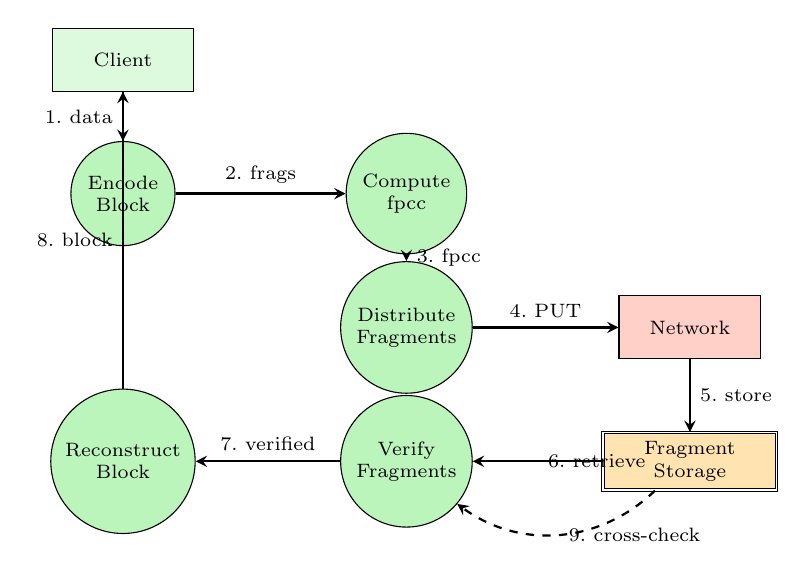
\begin{tikzpicture}[node distance=1.8cm]
  \node (client)      [entity, fill=trusted!30]      {Client};
  \node (encode)      [process, below of=client, yshift=0.1cm] {Encode\\Block};
  \node (fingerprint) [process, right of=encode, xshift=1.8cm] {Compute\\fpcc};
  \node (distribute)  [process, below of=fingerprint, yshift=0.1cm] {Distribute\\Fragments};
  \node (network)     [entity, fill=untrusted!30, right of=distribute, xshift=1.8cm] {Network};
  \node (storage)     [datastore, fill=semitrusted!30, below of=network, yshift=0.1cm] {Fragment\\Storage};
  \node (verify)      [process, below of=distribute, yshift=0.1cm] {Verify\\Fragments};
  \node (reconstruct) [process, left of=verify, xshift=-1.8cm] {Reconstruct\\Block};

  \draw[arrow] (client)      -- node[left,  font=\scriptsize] {1.~data}       (encode);
  \draw[arrow] (encode)      -- node[above, font=\scriptsize] {2.~frags}      (fingerprint);
  \draw[arrow] (fingerprint) -- node[right, font=\scriptsize] {3.~fpcc}       (distribute);
  \draw[arrow] (distribute)  -- node[above, font=\scriptsize] {4.~PUT}        (network);
  \draw[arrow] (network)     -- node[right, font=\scriptsize] {5.~store}      (storage);
  \draw[arrow] (storage)     -- node[right, font=\scriptsize] {6.~retrieve}   (verify);
  \draw[arrow] (verify)      -- node[above, font=\scriptsize] {7.~verified}   (reconstruct);
  \draw[arrow] (reconstruct) -- node[left,  font=\scriptsize] {8.~block}      (client);
  \draw[arrow,dashed] (storage) to[bend left=40]
        node[right, font=\scriptsize] {9.~cross-check} (verify);
\end{tikzpicture}
\caption{High-level data flow: green = trusted, orange = semi-trusted, red = untrusted.}
\label{fig:dfd}
\end{figure}

% ============================================================
\section{Implementation}

\subsection{Technology Stack}

\begin{center}
\small
\begin{tabular}{lll}
\hline
\textbf{Component} & \textbf{Library} & \textbf{Purpose} \\
\hline
Finite field arithmetic & \texttt{numpy} $\geq$ 1.26 & GF(256) polynomial ops \\
Erasure coding & custom (\texttt{src/erasure/}) & Cauchy-matrix RS encode/decode \\
REST API server & \texttt{fastapi} $\geq$ 0.110, \texttt{uvicorn} & Fragment storage endpoints \\
HTTP client & \texttt{httpx} $\geq$ 0.27 & Async parallel fragment dispersal \\
Data validation & \texttt{pydantic} $\geq$ 2.6 & Request/response schema enforcement \\
Testing & \texttt{pytest}, \texttt{pytest-asyncio} & Unit and integration tests \\
\hline
\end{tabular}
\end{center}

\vspace{0.3em}
\textbf{Design choice}: \texttt{fastapi} + \texttt{pydantic} was chosen because schema
validation happens automatically at the API boundary, rejecting malformed requests
(e.g., impossible parameters like $m > n$) before they reach storage logic.

\subsection{Module Architecture}

\begin{lstlisting}
src/
  erasure/      encoder.py, decoder.py, matrix.py  -- RS encode/decode
  fingerprint/  fingerprint.py, polynomial.py, field.py  -- GF(256) fp
  verification/ cross_checksum.py, oracle.py, verifier.py  -- fpcc + verify
  network/      client.py, server.py, protocol.py, rate_limit.py
  storage/      store.py, fragment.py, metadata.py
\end{lstlisting}

\subsection{Key Protocol: Dispersal (PUT)}

\begin{enumerate}
  \item \texttt{encoder.py} pads the input to a multiple of $m$ bytes, constructs the
        Cauchy matrix, and produces $n$ fragments as numpy arrays.
  \item \texttt{cross\_checksum.py} computes $\{h_i\}$, derives $r$ via
        \texttt{oracle.py}, and computes $\{\mathrm{fp}_i\}_{i<m}$ to produce the fpcc.
  \item \texttt{client.py} fans out $n$ parallel \texttt{httpx} PUT requests, each
        carrying the fragment (base64-encoded) and the serialized fpcc JSON.  A maximum
        of 3 retries with 0.5 s linear backoff handles transient failures.
  \item The server-side \texttt{server.py} immediately calls \texttt{Verifier.check()}
        on the received fragment before persisting it to disk.
\end{enumerate}

\subsection{Key Protocol: Retrieval (GET)}

\begin{enumerate}
  \item \texttt{client.py} issues $n$ parallel GET requests and collects the first $m$
        successful responses using \texttt{Thread\-Pool\-Executor}.
  \item For each returned fragment, \texttt{Verifier.check()} runs two checks:
        (a) \texttt{SHA-256} hash against the fpcc entry, and
        (b) for $i < m$, a fingerprint check: $\mathrm{fp}(r', d_i) \stackrel{?}{=}
            \mathrm{fpcc.fingerprints}[i]$.
  \item Only fragments that return \texttt{CONSISTENT} are passed to
        \texttt{decoder.py}, which inverts the Cauchy matrix to recover the original
        block and strips padding.
\end{enumerate}

% ============================================================
\section{Security Analysis}

\subsection{Trust Levels}

\textbf{Administrator}: Full access; assumed benign.
\textbf{Authenticated Client}: Verified identity; may run buggy software.
\textbf{Storage Server}: \emph{Semi-trusted} — may be compromised, return stale or
corrupted fragments, or attempt to forge data.
\textbf{Network}: Untrusted; adversary may observe, inject, or modify traffic.

\subsection{STRIDE Threat Summary}

\begin{center}
\small
\begin{tabular}{llp{5.5cm}l}
\hline
\textbf{ID} & \textbf{Category} & \textbf{Threat} & \textbf{Status} \\
\hline
S.1 & Spoofing   & Client impersonation via block ID        & Bearer token (partial) \\
S.2 & Spoofing   & Server impersonation; no TLS             & Accepted (localhost) \\
S.3 & Spoofing   & Forged fpcc from malicious server        & Requires mitigation \\
T.1 & Tampering  & Fragment corruption in storage           & \textbf{Mitigated} \\
T.2 & Tampering  & In-transit fragment modification         & Partially mitigated \\
T.3 & Tampering  & Coordinated fpcc + fragment forgery      & Requires mitigation \\
T.4 & Tampering  & Erasure code parameter manipulation      & Partially mitigated \\
R.2 & Repudiation& Fragment deletion without audit trail    & \textbf{Mitigated} \\
I.1 & Info.\ disc.& Fragment eavesdropping (no TLS)        & Dependency (TLS) \\
I.4 & Info.\ disc.& Verbose error message leakage          & \textbf{Mitigated} \\
\hline
\end{tabular}
\end{center}

\subsection{Core Security Guarantee}

Theorem 3.4 (Hendrics et al.) bounds the miss probability of the fingerprint check at
$\leq 1/|\mathrm{GF}(256)| = 1/256$ per check.  Empirically, testing all single-byte
flips across 100 blocks ($\times$5 fragments each) yielded a \textbf{100\% detection
rate} and a \textbf{0.0\% false positive rate}.  The system tolerates up to $n - m = 2$
Byzantine faults: as long as $\geq 3$ honest servers are available, the client recovers
the original block correctly.

% ============================================================
\section{System Behavior}

\subsection{Expected Behavior: Honest Operation}

A typical session starts 5 server processes on \texttt{localhost:5001}--\texttt{5005},
then uses the client to store and retrieve a file:

\begin{lstlisting}[language=bash]
# Start servers (each on a distinct port)
$ uvicorn src.network.server:app --port 5001 &
...
# Store a file
$ python -m src.network.client store myfile.bin
Dispersed block abc123 to 5/5 servers.  fpcc stored.
# Retrieve the file
$ python -m src.network.client retrieve abc123
Retrieved 3/5 fragments; all verified CONSISTENT.
Reconstructed 4096 bytes -> myfile_out.bin
\end{lstlisting}

\subsection{Expected Behavior: Byzantine Server}

When a server returns a corrupted fragment, the verifier rejects it and the client falls
back to an honest server:

\begin{lstlisting}
[WARNING] server_2: HASH_MISMATCH for block abc123 fragment 1 (index 1)
[INFO]    Fragment 1 rejected; trying server_4...
[INFO]    Retrieved 3 verified fragments from servers 0, 3, 4.
[INFO]    Reconstructed successfully.
\end{lstlisting}

\subsection{Expected Behavior: Too Many Failures}

If more than $n - m = 2$ servers are lost, the client fails closed with a clear error:

\begin{lstlisting}
[ERROR] Only 2 verified fragments available; need 3.  Raising RetrievalError.
RetrievalError: Insufficient verified fragments for block abc123.
\end{lstlisting}

\subsection{Test Suite Results}

The security test suite covers verification-layer unit tests, HTTP endpoint tests, and
full integration tests wiring a live \texttt{VeriStoreClient} to multiple in-process
server instances.

\begin{itemize}
  \item \textbf{Unit tests}: all byte-flip mutations on test fragments detected;
        \texttt{HASH\_MISMATCH} or \texttt{FP\_MISMATCH} returned in every case.
  \item \textbf{Endpoint tests}: malformed base64, impossible parameters
        ($m > n$), duplicate PUT, and missing bearer token all return the correct
        HTTP error codes (400, 409, 422, 401).
  \item \textbf{Integration tests}: end-to-end store/retrieve with 0, 1, and 2
        Byzantine servers; failure with 3 Byzantine servers confirmed.
  \item \textbf{Empirical experiments}: collision-probability experiment over 500 checks
        confirms $\leq 1/256$ theoretical bound; false positive rate = 0.0\%.
\end{itemize}

\end{document}
